
We detail our contributions, and the corresponding software features next.

\vspace{-5pt}
\subsection{A model-free parametrization}

We identify the core parameters common to models of qualitative traits,
\begin{itemize}
    \item Sample sizes, i.e., the number of Cases, $n_1$, and Controls, $n_2$,
    \item Conditional distribution of risk variant among Controls, i.e., risk allele frequency (RAF) in the Control group, denoted $f$.
    \item Odds ratio (OR) of genotype variants, denoted $\text{R}$.
\end{itemize}
An alternative hypothesis, e.g., a disease model, determines the set of quantities either implicitly or explicitly,
and therefore determines statistical power for a given test procedure.
% From a statistical perspective, the disease model serves no role except to specify the distribution of the counts under the alternative.
In the software, statistical power is calculated directly based the quartet $(n_1, n_2, f, R)$, allowing us to perform model-free analysis, valid for studies employing different models.

We make the important distinction here between RAF \emph{in the Control group} ($f$), versus RAF \emph{in the study}, and RAF \emph{in the general population}.
Throughout this work, RAF refers to the risk allele frequency in the Control group, consistent with the reporting standard of the NHGRI-EBI Catalog.

\vspace{-5pt}
\subsection{A test-independent power analysis}

While power calculations are necessarily tied to the statistical tests used, fortunately, for many common association tests, statistical powers are asymptotically equivalent.
It is perhaps well-known that for tests of associations in contingency tables, the likelihood ratio (LR) test and Pearson's chi-square test enjoy the same the same power asymptotically.
We further show that tests including, e.g., Welch's t-test (though not student t-test) and LR tests for logistic regressions, also have asymptotically the same power, as long as the core parameters assume the same values.
Our model-free, test-independent analysis allows us to calculate power in a unified fashion. 
The theoretical analysis, and formulas for power calculations in terms of the core parameters, are detailed in the Supplementary material.

In the software, end users need only prescribe the sample sizes. 
The common power limits are calculated as a function of RAF and OR, and visualized as a heatmap in the OR-RAF diagram; see Figure \ref{fig:02} for a preview of the software graphical user interface.

\begin{figure}[!tpb]%figure1
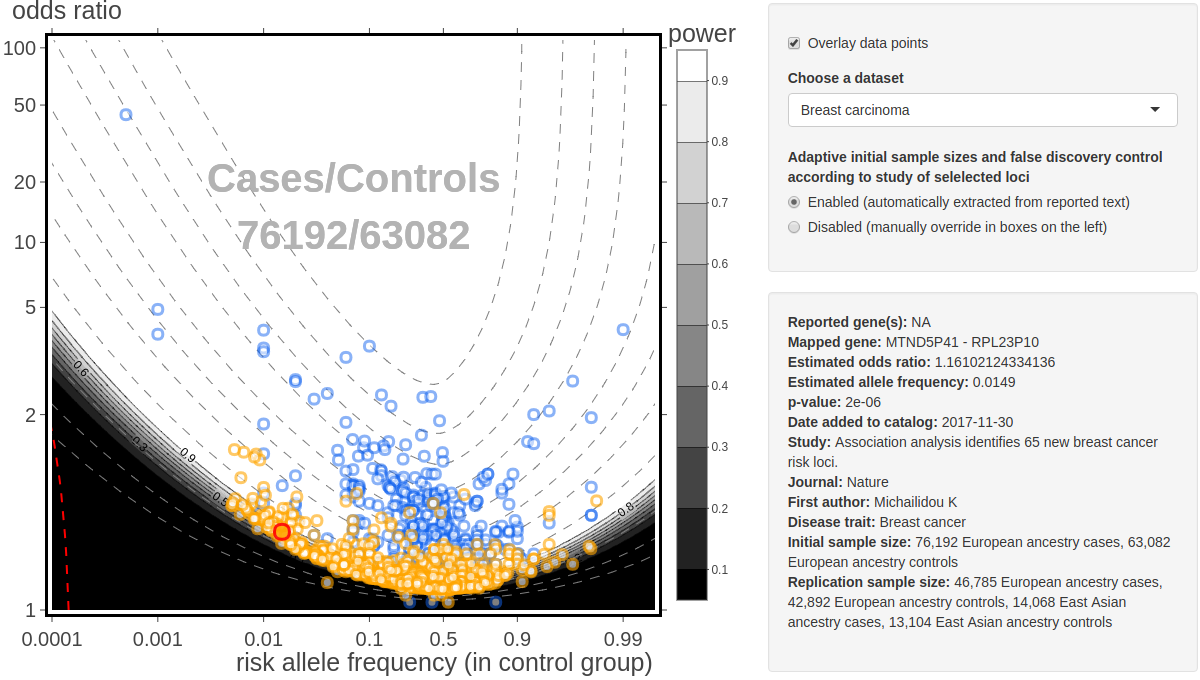
\includegraphics[width=0.48\textwidth]{Screenshot_GWAS_calculator6.png}
\vspace{-20pt}
\caption{Snapshot of the interactive application's forensics functionality, illustrated with all findings from breast cancer studies reported in the NHGRI-EBI GWAS Catalog (circles),
% the reported odds ratios and risk allele frequencies in the control groups. 
overlaid on the OR-RAF power diagram of association tests (greyscale heatmap).
The initial sample sizes are dynamically adjusted, and automatically determined from texts of the article reporting the user selected genes (red circle). 
Information of the selected genes and the articles are also dynamically displayed; findings reported in the same article are highlighted (orange circles).
We provide finite sample corrections by marking the rare variant region(s) (red dashed lines).
}\label{fig:02}
\end{figure}

\vspace{-5pt}
\subsection{Review and forensics of reported findings}

This unified treatment allows us to examine results from different studies employing different models and applicable tests, in the \emph{same} diagram, with the \emph{same} power limits.
It allows for a systematic review of reported findings for their statistical validity. 
In particular, a reported association predicted to have low power (i.e., probability of discovery) at the study's sample size (lying in the dark regions of the OR-RAF diagram), while not impossible, should invite further investigations. {It should also be noted that a reported association predicted to have high power is not automatically accurate -- other forms of errors, such as selection bias, may inflate OR and RAF estimates.}

The software provides options for the users to load and overlay findings reported in the NHGRI-EBI GWAS Catalog, or alternatively, upload data from other sources, 

% In particular, for large samples, tests for zero slopes in logistic regressions should report approximately the same set of loci as Welch's t-tests for equal proportions on the same dataset, after the same family-wise error rate adjustments.
% The estimated odds ratios (in the case of logistic regression, estimate slopes exponentiated) and RAF's, when charted on the OR-RAF diagram, should also follow the same power limits.


\vspace{-5pt}
\subsection{Rare variant and finite sample corrections}

We explicitly address the quality of asymptotic approximations in our power analysis, and the applicability of single-SNP-based tests when rare genetic variants are present.
Specifically, provide a lower bound on the variant counts necessary for Fisher's exact test to be calibrated to have the desired type I, or family-wise, error rate. 
If rare variant counts fall below the threshold, the asymptotic approximations do not apply.
In such cases, exact tests, and by extension, single-SNP-based association tests, cannot be correctly calibrated without sacrificing all statistical power.
We mark this low-count, zero-power region on the OR-RAF diagram.

We also provide options for users to specify the rare variant as 1) having less than a specified counts, or 2) occurring in less than a percentage of all subjects in the study, as is customary in the literature.



